\documentclass[14pt, a4paper]{article}
\usepackage{minitoc}
\usepackage[left=3.00cm, right=2.5cm, top=2.00cm, bottom=2.00cm]{geometry}
\usepackage{amsmath}
\usepackage{amssymb}
\usepackage{amsthm}
\usepackage{thmtools}
\usepackage{mathtools}
\usepackage{graphicx}
%\usepackage{algpseudocode}
%\usepackage{algorithm}
\usepackage[ruled,vlined,linesnumbered,algosection]{algorithm2e}
\usepackage{blindtext}
\usepackage{setspace}
\usepackage[utf8]{inputenc}
\usepackage[utf8]{vietnam}
\usepackage[center]{caption}
\usepackage[shortlabels]{enumitem}
\usepackage{fancyhdr} % header, footer
\usepackage{hyperref} % loại bỏ border với mục lục và công thức
\usepackage[nonumberlist, nopostdot, nogroupskip]{glossaries}
\usepackage{glossary-superragged}
\usepackage{tikz,tkz-tab}
\setglossarystyle{superraggedheaderborder}
\pagestyle{fancy}
%\usepackage[style=numeric,sortcites]{biblatex}
%\addbibresource{ref.bib}
%\usepackage[numbers]{natbib}
\usepackage{indentfirst}
\usepackage{multirow}
\usepackage[natbib,backend=biber,style=ieee, sorting=ynt]{biblatex}
\bibliography{ref.bib}

\graphicspath{{./figures/}}


\makenoidxglossaries

% Danh mục thuật ngữ

\hypersetup{
    colorlinks=false,
    pdfborder={0 0 0},
}


\fancyhf{}
\rhead{\textbf{Môn học: Một số vấn đề về đồ họa máy tính}}
\lhead{\textbf{GVHD: TS. Nguyễn Thị Bích Thủy}}
\rfoot{\thepage}
\lfoot{\textbf{Học viên thực hiện: Nguyễn Chí Thanh - 21007925}}
\renewcommand{\headrulewidth}{0.4pt}
\renewcommand{\footrulewidth}{0.4pt}


\numberwithin{equation}{section}
\numberwithin{figure}{section}

\setlength{\parindent}{0.5cm}

\setcounter{secnumdepth}{3} % Cho phép subsubsection trong report
\setcounter{tocdepth}{3} % Chèn subsubsection vào bảng mục lục

\newtheorem{dl}{Định lý}
\newtheorem{md}{Mệnh đề}
\newtheorem{bd}{Bổ đề}
\newtheorem{dn}{Định nghĩa}
\newtheorem{hq}{Hệ quả}

\numberwithin{dl}{section}
\numberwithin{md}{section}
\numberwithin{bd}{section}
\numberwithin{dn}{section}
\numberwithin{hq}{section}

\doublespacing
\AtBeginEnvironment{tabular}{\doublespacing}

\begin{document}
    \begin{titlepage}

        \newcommand{\HRule}{\rule{\linewidth}{0.5mm}} % Defines a new command for the horizontal lines, change thickness here

        \center % Center everything on the page

        %----------------------------------------------------------------------------------------
        %	HEADING SECTIONS
        %----------------------------------------------------------------------------------------
        \textsc{\LARGE Đại học Quốc Gia Hà Nội}\\[0.5cm]
        \textsc{\LARGE Trường đại học Khoa học tự nhiên}\\[0.5cm] % Name of your university/college
        \textsc{\LARGE Khoa Toán - Cơ - Tin học}\\[0.5cm]

        
\includegraphics[scale=0.2]{HUS-logo.jpg}\\[0.5cm]

        \textsc{\Large Chuyên ngành: Khoa học dữ liệu}\\[0.5cm] % Major heading such as course name


        %----------------------------------------------------------------------------------------
        %	TITLE SECTION
        %----------------------------------------------------------------------------------------

        \HRule \\[0.4cm]
        { \huge \bfseries BÀI TẬP MÔN HỌC}\\[0.4cm] % Title of your document
        \HRule \\[1.5cm]

        \textsc{\Large Môn học: Một số vấn đề về đồ họa máy tính}\\[1cm] % Minor heading such as course title


        \textsc{\Large Đề tài: Trực quan hóa văn bản và tài liệu}\\[2cm]


        %----------------------------------------------------------------------------------------
        %	AUTHOR SECTION
        %----------------------------------------------------------------------------------------
        \begin{minipage}{0.4\textwidth}
            \begin{flushleft} \large
            \emph{Giảng viên hướng dẫn:} \\
            TS. Nguyễn Thị Bích Thủy % Supervisor's Name
            \end{flushleft}
        \end{minipage}\\[0.5cm]

        \begin{minipage}{0.4\textwidth}
        \begin{flushleft} \large
        \emph{Học viên thực hiện:}\\
        Nguyễn Chí Thanh \\
        MSHV: 21007925 \\ % Your name
        Lớp: Khoa học dữ liệu - K4
        \end{flushleft}
        \end{minipage}


        % If you don't want a supervisor, uncomment the two lines below and remove the section above
        %\Large \emph{Author:}\\
        %John \textsc{Smith}\\[3cm] % Your name

        %----------------------------------------------------------------------------------------
        %	DATE SECTION
        %----------------------------------------------------------------------------------------

        % I don't want day because it is English
        % {\large \today}\\[2cm] % Date, change the \today to a set date if you want to be precise

        %----------------------------------------------------------------------------------------
        %	LOGO SECTION
        %----------------------------------------------------------------------------------------

        %\includegraphics{logo/rsz_3logo-khtn.png}\\[1cm] % Include a department/university logo - this will require the graphicx package

        %----------------------------------------------------------------------------------------

        \vfill % Fill the rest of the page with whitespace

    \end{titlepage}

    \cleardoublepage
    \pagenumbering{gobble}
    \tableofcontents
    \newpage
    \listoffigures
    \newpage
    \glsaddall 
    \renewcommand*{\glossaryname}{Danh mục các từ viết tắt}
    \renewcommand*{\acronymname}{Danh sách từ viết tắt}
    \renewcommand*{\entryname}{Viết tắt}
    \renewcommand*{\descriptionname}{Viết đầy đủ}
    \printnoidxglossary
    \cleardoublepage
    \pagenumbering{arabic}

    %\maketitle

    \newpage

    \nocite{*}

    \begin{center}
    \section*{LỜI MỞ ĐẦU}
    \end{center}
    \addcontentsline{toc}{section}{{\bf LỜI MỞ ĐẦU}\rm}

    Ta có một nguồn tài nguyên thông tin khổng lồ; từ các thư viện, đến các bộ lưu trữ email,
    đến tất cả các khía cạnh của các ứng dụng trên internet.
    Trực quan hóa là một công cụ tuyệt vời để phân tích các dữ liệu này.
    Ta có thể trực quan hóa theo nhiều dạng dữ liệu như blog, wiki, twitter feed,
    hàng tỷ từ, một tập các tờ báo hoặc một thư viện số.
    Trực quan hóa dữ liệu là một công việc phụ thuộc theo nghĩa là các công việc nào phù hợp với văn bản, tài liệu hoặc các đối tượng liên quan đến web.
    Cho dữ liệu văn bản và tài liệu, hầu hết các nhiệm vụ liên quan là tìm một từ, một cụm từ hoặc một chủ đề.
    Với dữ liệu có cấu trúc một phần, ta có thể tìm kiếm mối quan hệ giữa các từ, các cụm từ, các chủ đề hoặc giữa các tài liệu.
    Với văn bản hoặc tài liệu, nhiệm vụ chính và phổ biến nhất thường là tìm các mẫu và các điểm ngoại lai trong văn bản hoặc tài liệu.

    Đề tài này ta sẽ tập trung vào nhiệm vụ trực quan hóa dữ liệu dạng văn bản và các phương pháp tiếp cận để phân tích trực quan dữ liệu văn bản.

    \newpage

    \section{Mở đầu}

    Ta định nghĩa một tập các tài liệu là một \textit{corpus} (số nhiều là \textit{corpora}).
    Ta làm việc với các đối tượng trong corpora.
    Các đối tượng này có thể là các từ, các câu, đoạn văn, tài liệu hoặc một tập các tài liệu.
    Ta có thể xem xét cả các ảnh và video.
    Các đối tượng trên thường được xem là nguyển tử tương ứng với các nhiệm vụ, phân tích và trực quan hóa.
    Văn bản và tài liệu thường được ở dạng có cấu trúc tối thiểu và rất đa dạng các thuộc tính và metadata,
    đặc biệt khi ta tập trung vào một lĩnh vực ứng dụng cụ thể.
    Ví dụ, các tài liệu có một định dạng và thường bao gồm metadata về tài liệu (ví dụ tác giả, ngày được tạo, ngày sửa đổi, bình luận, kích thước).
    Các hệ thống truy hồi thông tin thường được dùng để truy vấn corpora, thường yêu cầu tính toán độ phù hợp của tài liệu ứng với một truy vấn.
    Nhiệm vụ này yêu cầu tiền xử lý tài liệu và sự giải thích về ngữ nghĩa của văn bản.

    Ta có thể tính toán thống kê về tài liệu.
    Ví dụ, số lượng các từ hoặc đoạn văn hoặc phân phối của các từ hoặc tần suất của các tự, tất cả có thể được sử dụng để xác thực tác giả.
    Câu hỏi là liệu có đoạn văn nào được lặp lại với cùng các từ và các câu?
    Ta có thể xác định mối quan hệ giữa các đoạn văn hoặc mối quan hệ giữa các tài liệu trong một corpus.
    Ví dụ, khi một người hỏi, "Những tài liệu nào liên quan đến sự lây lan của dịch cúm?"
    Đây không phải là một câu truy vấn đơn giản, ta không thể đơn giản tìm kiếm cho từ "cúm" hay "dịch cúm".
    Ta cần phải xem xét đến sự kết nối và các mối quan hệ giữa nhiều tài liệu rằng có tồn tại các cụm không?
    Các tài liệu này có trình bày về chủ đề đang tìm kiếm trong corpus không?
    Sự tương đồng có thể được định nghĩa trong quan hệ về trích dẫn, quyền tác giả, các chủ đề,\dots

    \section{Các cấp của biểu diễn văn bản}

    Ta định nghĩa ba cấp độ biểu diễn văn bản: từ vựng, cú pháp và ngữ nghĩa.
    Mỗi cấp độ biểu diễn đều yêu cầu chuyển đổi văn bản từ dạng phi cấu trúc sang dạng dữ liệu có cấu trúc.

    \textbf{Cấp độ từ vựng.} Cấp độ từ vựng liên qua đến việc biến đổi một chuỗi các ký tự sang một dãy các thực thể nguyên tử được gọi là \textit{tokens}.
    Bộ phân tích từ vựng xử lý dãy các ký tự với một bộ quy tắc nhất định thành một dãy các tokens mới có thể được sử dụng cho những phân tích sâu hơn.
    Tokens có thể bao gồm các ký tự, các ký tự n-grams, các từ, các gốc từ, các từ vựng, các cụm từ, hoặc các từ n-grams, với tất cả các thuộc tính liên quan.
    Nhiều kiểu quy tắc có thể được dùng để trích xuất các tokens, phổ biến nhất là máy trạng thái hữ hạn được xác định bởi các biểu thức chính quy.

    \textbf{Cấp độ cú pháp.} Cấp độ cú pháp liên quan đến việc xác định và gắn thẻ (chú thích) cho từng chức năng của tokens.
    Ta chỉ định nhiều thẻ khác nhau, chẳng hạn vị trí câu hoặc một từ là danh từ hay tục ngữ, tính từ, bổ ngữ, liên từ hay không.
    Tokens có thể có các thuộc tính như là số ít hoặc số nhiều, sự tương đồng với các tokens khác.
    Các thẻ đa dạng hơn bao gồm ngày, lượng tiền, địa điểm, cá nhân, tổ chức và thời gian (hình \ref{fig:3}).
    Quá trình trích xuất các gán nhãn này được gọi là \textit{nhận diện thực thể được đặt tên} (NER).
    Sự phong phú và đa dạng của các mô hình ngôn ngữ và ngữ pháp (mô hình sinh, mô hình phân loại, phụ thuộc, xác suất và chức năng luận) mang lại nhiều cách tiếp cận khác nhau.

    \textbf{Cấp độ ngữ nghĩa.} Cấp độ ngữ nghĩa bao gồm việc trích xuất xuất các ý nghĩa và quan hệ giữa các phần tri thức thu được từ các cấu trúc được xác định ở cấp độ cú pháp.
    Mục tiêu của cấp độ này là xác định một giải thích phân tích của toàn văn bản trong một ngữ cảnh cụ thể hoặc thậm chí không phụ thuộc vào ngữ cảnh.

    \section{Mô hình không gian vector}

    Tính toán vectors các thuật ngữ hoặc các từ là một bước thiết yếu cho nhiều kỹ thuật trực quan hóa và phân tích tài liệu và văn bản.
    Trong \textit{mô hình không gian vector} \cite{356}, một vector của một thuật ngữ hoặc một từ cho một đối tượng quan tâm (đoạn văn, tài liệu hoặc một tập các tài liệu) là một vector mà trong đó mỗi chiều biểu diễn trọng số của một từ đã cho trong tài liệu đó.
    Thông từ, để loại bỏ nhiễu hoặc các từ dừng (stop words) (ví dụ "the", "a") được loại bỏ (lọc) và các từ có chung gốc được ghép vào làm một (ghép từ gốc).

    Mã giả bên dưới đếm số lần xuất hiện của các tokens riêng biệt, ngoại trừ các từ dừng.
    Đầu vào được giả định là một luồng của các tokens được tạo ra bởi bộ phân tích từ vựng cho một tài liệu.
    Biến các thuật ngữ bao gồm một bảng băm ánh xạ các thuật ngữ riêng biệt với số lượng của chúng trong tài liệu.

    \begin{algorithm}[h!]
        \DontPrintSemicolon
        $terms \gets \emptyset$\;
        \ForEach{$token$ $t$ \textbf{in} $tokenStream$}{
            \If{$t$ không phải là một từ dừng}{
                \If{$t$ \textbf{not in} $terms$} {
                    $terms \lbrack t \rbrack \gets 1$\;
                } 
                \Else {
                    $terms \lbrack t \rbrack \gets terms \lbrack t \rbrack + 1$\;
                }
            }
        }
        \Return{$terms$}\;
        \caption{COUNT-TERMS(tokenStream)}
        \label{alg:COUNT-TERMS}
    \end{algorithm}

    Ta áp dụng mã giả thuật toán \ref{alg:COUNT-TERMS} cho đoạn văn dưới đây:
    
    \begin{verbatim}
        There is a great deal of controversy about the safety of genetically
    engineered foods. Advocates of biotechnology often say that the risks
    are overblown. ‘‘There have been 25,000 trials of genetically
    modified crops in the world, now, and not a single incident, or
    anything dangerous in these releases,’’ said a spokesman for Adventa
    Holdings, a UK biotech firm. During the 2000 presidential campaign,
    then-candidate George W. Bush said that ‘‘study after study has shown
    no evidence of danger.’’ And Clinton Administration Agriculture
    Secretary Dan Glickman said that ‘‘test after rigorous scientific
    test’’ had proven the safety of genetically engineered products.
    \end{verbatim}

    Đoạn văn trên bao gồm 98 tokens, 74 thuật ngữ và 48 thuật ngữ khi các từ dừng được loại bỏ.
    Đây là một mẫu của vector thuật ngữ được tao ra từ thuật toán \ref{alg:COUNT-TERMS}:

    \begin{table}[h!]
        \begin{tabular} {|c| c| c| c| c| c| c| c| c| c|}
            \hline
            genetically & said & safety & engineered & study & test & great & deal & controversy & foods \\
            \hline
            3 & 3 & 2 & 2 & 2 & 2 & 1 & 1 & 1 & 1 \\
            \hline
        \end{tabular}
    \end{table}

    \begin{figure}[h!]
        \centering
        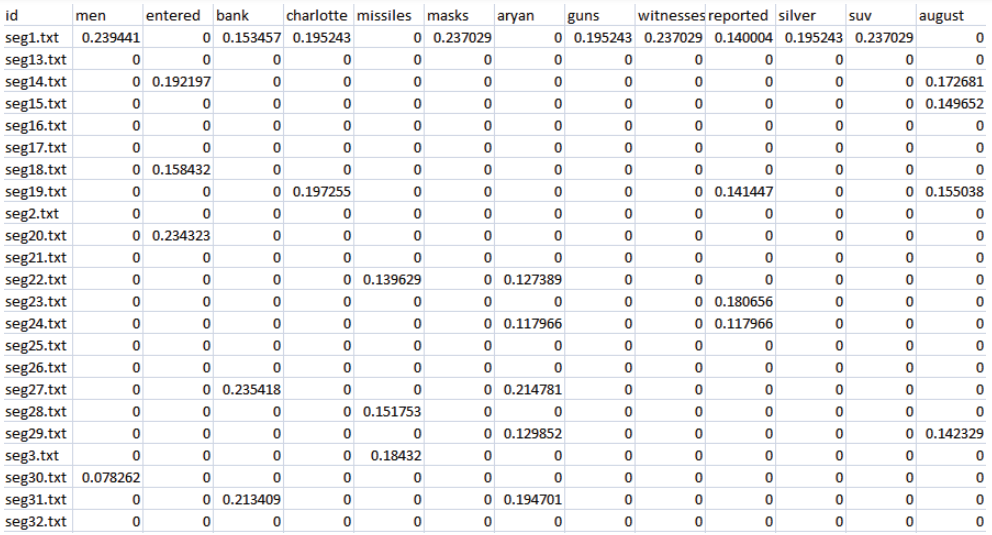
\includegraphics[width=0.8\textwidth]{1.png}
        \caption{Minh họa của các vector của các thuật ngữ trong nhiều tài liệu, bao gồm giá trị tf-idf.}
    \end{figure}

    \begin{algorithm}[h!]
        \DontPrintSemicolon
        $termFrequencies \gets \emptyset$\; \tcp{Tra cứu bảng đếm số lần thuật ngữ/từ xuất hiện cho tên tài liệu}
        $documentFrequencies \gets  \emptyset$\; \tcp*{Đếm số tài liệu mà trong đó một thuật ngữ/từ nhất định xuất hiện}
        $uniqueTerms \gets \emptyset$\; \tcp*{Danh sách các thuật ngữ/từ riêng biệt}
        \ForEach{$document$ $d$ \textbf{in} $documents$}{
            $docName \gets NAME(d)$\; \tcp{Trích xuất tên của tài liệu}
            $tokenStream \gets TOKENIZE(d)$\; \tcp{Tạo luồng token của tài liệu}
            $terms \gets COUNT-TERMS(tokenStream)$\; \tcp{Đếm tần suất của các thuật ngữ/từ}
            $termFrequencies \lbrack docName \rbrack \gets terms$\; \tcp{Lưu trữ tần suất các thuật ngữ/từ tương ứng với từng tài liệu}
            \ForEach{$term$ $t$ \textbf{in} $KEYS(terms$)}{
                \If{$t$ \textbf{not in} $documentFrequencies$} {
                    $documentFrequencies \lbrack t \rbrack \gets 1$\;
                } 
                \Else {
                    $documentFrequencies \lbrack t \rbrack \gets documentFrequencies \lbrack t \rbrack + 1$\;
                }
                $uniqueTerms \gets uniqueTerms \cup t$\;
            }
        }
        $tfIdfVectorTable \gets \emptyset$\; \tcp{Tra cứu vector tf-idf cho tên tài liệu}
        $n \gets LENGTH(documents)$\;
        \ForEach{$document$ $name$ $docName$ \textbf{in} $KEYS(termFrequencies)$}{
            $tfIdfVector \gets $ \text{zeroes array of length} $LENGTH(uniqueTerms)$\;
            $terms \gets termFrequencies \lbrack docName \rbrack$\;
            \ForEach{$term$ $t$ \textbf{in} $KEYS(terms)$}{
                $tf \gets terms \lbrack t \rbrack$\;
                $df \gets documentFrequencies \lbrack t \rbrack$\;
                $tfIdf \gets tf \times \log \Big( \dfrac{n}{df} \Big)$\;
                $tfIdfVector \lbrack \text{chỉ số của } t \text{ trong } uniqueTerms \rbrack \gets tfIdf$\;
            }
            $tfIdfVectorTable \lbrack docName \rbrack \gets tfIdfVector$\;
        }
        \Return{$tfIdfVectorTable$}\;
        \caption{COMPUTE-TFIDF(documents)}
        \label{alg:COMPUTE-TFIDF}
    \end{algorithm}

    \begin{figure}[h!]
        \centering
        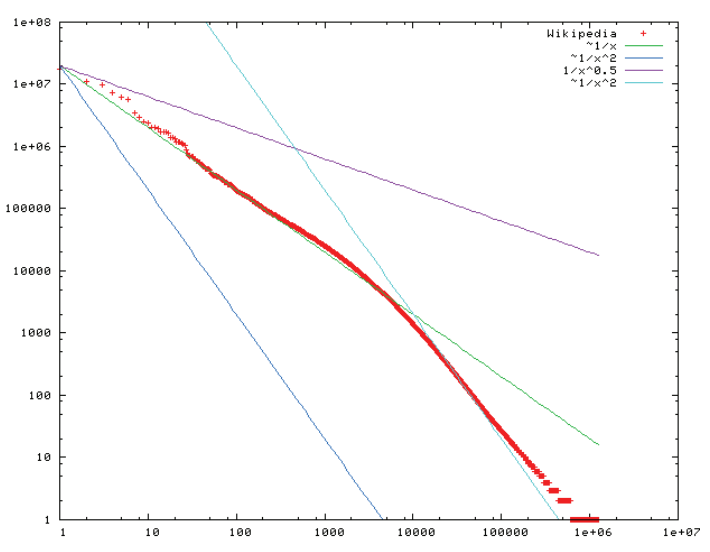
\includegraphics[width=0.8\textwidth]{2.png}
        \caption{Phân phối của các thuật ngữ trong Wikipedia, một ví dụ về luật Zipf.
        Phân phối của các thuật ngữ nằm trên trục y, và thứ hạng tần suất nằm trên trục x.}
    \end{figure}


    \begin{figure}[h!]
        \centering
        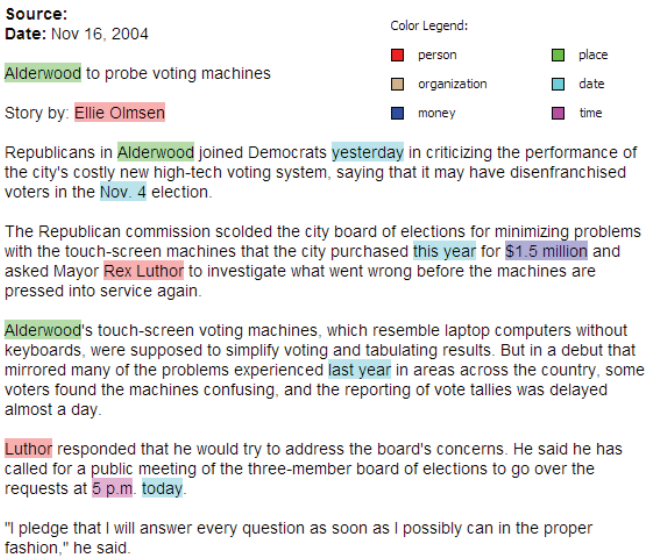
\includegraphics[width=0.8\textwidth]{3.png}
        \caption{Chế độ xem mà các thực thể có tên được tô sáng, các màu tô sáng tương ứng theo loại thực thể}
        \label{fig:3}
    \end{figure}


    \newpage
    
    \printbibliography[title={TÀI LIỆU THAM KHẢO}]
\end{document}